\section{Designs}
The two main features to be designed in this project are the gameplay itself,
and the user interface.

\subsection{Gameplay Design}
In this section a high level description of the gameplay will be outlined.
This can be seen in Algorithm~\ref{code:pokerServer}

\vspace{0.3cm}

\begin{algorithm}[H]
    \nlset{STEP 1} start server\;
    \nlset{STEP 2} wait for minimum connections\;
    \nlset{STEP 3} launch game\;
    \While{players $>$ 1}{
        \nlset{STEP 4} deal cards to each player\;
        \For{each betting round while (players in play $>$ 1)}{
            \nlset{STEP 5} prompt each player for action\;
            evaluate actions\;
            \nlset{STEP 6} reveal next set of cards\;
        }
        \nlset{STEP 7} update player chips counts\;
        remove players with no chips\;
    }
\caption{The poker server algorithm}%
\label{code:pokerServer}
\end{algorithm}

\vspace{0.3cm}

We can now talk about each step of the implementation in more detail, and the
problems encountered. Once a player connects to the server, upon receiving
an initial message from the server, the developed client then launches
a GUI, which is talked about more in depth in its relevant section. Once the
GUI is launched, the initial two cards are dealt to every player. Card dealing 
has been abstracted, and as mentioned in the randomness section, is adaptable, 
and supports multiple different card picking and randomness sources. A new deck
is initiated each round, with the chosen card picking and randomness sources. 
There are currently three different methods of picking a card.

\begin{itemize}
    \item Knuth Shuffle
    \item Random Indexing
    \item Random Sorting Shuffle
\end{itemize}

The knuth shuffle \parencite{knuth1997} can be implemented as in
Algorithm~\ref{code:knuthShuffle}

\vspace{0.3cm}

\begin{algorithm}[H]
    \SetKwInOut{Input}{input}\SetKwInOut{Output}{output}
    \Input{An array $xs$ of cards, a function $getRandomNumber$ that takes an
           int, and returns a random number between 0 and this int}
    \Output{$xs$ shuffled}
    \BlankLine{}
    \For{$i \leftarrow length (xs) - 1$ \KwTo{} 1}{
        \nlset{STEP 1} $j \leftarrow getRandomNumber (i)$\;
        \nlset{STEP 2} swap ($xs$, $i$, $j$)\;
    }
    \nlset{STEP 3} return $xs$\;
\caption{The knuth shuffle algorithm}%
\label{code:knuthShuffle}
\end{algorithm}

\vspace{0.3cm}

This algorithm produces uniformly distributed permutations, assuming the
getRandomNumber function produces random numbers between 0 and i. However,
a very similar version, which instead of swapping between i and j, swaps
between 0 and j is not uniformly distributed. This can be proven by
the fact that there are $n^n$ possible sequences of random numbers, whereas
there are ${n!}$ possible permutations, which is not a factor of $n^n$.
The knuth shuffle however can produce exactly ${n!}$ possible random number
sequences. \parencite{website:rici2015}

The second algorithm, Random Indexing, is very simple, and simply involves 
taking a random number r between 0, and the length of the card deck, and 
removing item r from the array. The random sorting shuffle however is less 
simple and again is described in algorithm~\ref{code:randomSortShuffle}

\vspace{0.3cm}

\begin{algorithm}[H]
    \SetKwInOut{Input}{input}\SetKwInOut{Output}{output}
    \Input{An array $xs$ of cards, a function $getRandomNumber$ that takes an
           int, and returns a random number between 0 and this int}
    \Output{$xs$ shuffled}
    \BlankLine{}
    \nlset{STEP 1} $randomNums \leftarrow []$\;
    \nlset{STEP 2} \For{$i \leftarrow 0$ \KwTo{} length ($xs$) $- 1$}{
        randomNums += getRandomNumber (${2}^{32}$)\;
    }
    \nlset{STEP 3} $combined \leftarrow zip$ (xs, randomNums)\;
    $sorted \leftarrow sortBy ( combined, compare (snd))$\;
    \nlset{STEP 4} return map (fst, $sorted$)\;
\caption{The random sort shuffle algorithm}%
\label{code:randomSortShuffle}
\end{algorithm}

\vspace{0.3cm}

The above algorithm generates a random number for each card, and assigns
one to each in a list of tuples. The list is then sorted by the random numbers,
and the random numbers are then thrown away, and the list is returned. One
possible pitfall of this algorithm is if the numbers generated are the same,
however the probability of this happening is very small, and is discussed
in the randomness section.

After cards have been dealt, each player in turn provides an action, these are
then evaluated on the server, one by one, affecting the actions the subsequent
players can then make. Action evaluation is done by simply updating a state 
monad which is threaded between all the main functions. For example, if a 
player makes a raise action, the minimum raise will be updated, the current bet 
will be updated, and the players bet and chips will be updated. These actions 
are propagated to the clients when necessary to update their GUI's. Unlike a 
global variable, a state monad is a pure function, taking an old state and 
returning a new state. The makes the code a lot easier to reason about, being 
able to test out individual functions in the Haskell GHCI interpreter with a 
custom state inputted, rather than having to run a complex series of functions 
to get the global state in a suitable condition to test the functionality. 
The state monad is also using the StateT monad transformer. This allows us to 
use IO impure functions whilst still remaining in the state monad. Due to the
setup of our type signatures, pure code is still in the StateT monad, but
has an abstract type signature, so is prevented from running IO effectful code.
In this way, we maintain ease of use, being able to call pure code in IO
functions without unwrapping or lifting state monads, whilst being able to
indicate impure functions in the type signature.

Once evaluation has finished, the server will then send a message back to the
client with a new state, which the client uses to update the GUI and
potentially prompt the player for a new action. To send these messages back
and forth, the two programs interact using the network library, which uses low 
level sockets to send messages to each other. The messages are queued and 
decoded one at a time on either side, as multiple messages can be packed into 
one read for efficiency. The messages are encoded with an efficient binary 
protocol to reduce the amount of data needing to be sent over the network. 
Even without these optimisations, due to the data being essentially text, the 
bandwidth needed to transfer the messages is very minimal. In the client, upon 
receiving a message, it will decode it, and depending upon the message type, 
it will generally update the internal state of the gameplay, then update the 
GUI to reflect these changes. Upon being prompted for an input, the related 
dialog boxes or buttons will be enabled and visible. Once an input is selected, 
this will be encoded and sent back to the server.

All inputs are validated on the server. This prevents malicious or faulty
clients from sending illegal or invalid messages which could alter their
standings or possibly crash the server. However, currently messages are not
encrypted went they are sent, which could allow malicious parties to man in the
middle the connection and alter the players actions. In future, we could look
into possible encryption techniques to secure this avenue of exploitation.

These few simple steps are essentially all that is needed to implement the
game of poker. It is worth noting that the proposed AI will work in nearly the 
exact same way as the client. A framework will be developed which takes care of 
updating the internal state and passing the messages back and forth, so all 
that is needed to create a new AI is to implement a function which takes a list
of valid inputs, and the current states, and returns a valid action. This will
enable very simple AI to be implemented in very few lines of code. For example,
an AI could be implemented which simply picks a random action and a random 
raise size, if raise is selected, could easily be implemented in 10 lines of
code.

\subsection{Graphical User Interface Design}
Designing the graphical interface began with simple mockups. A simple
initial diagram is shown below.

\begin{figure}[h]
    \frame{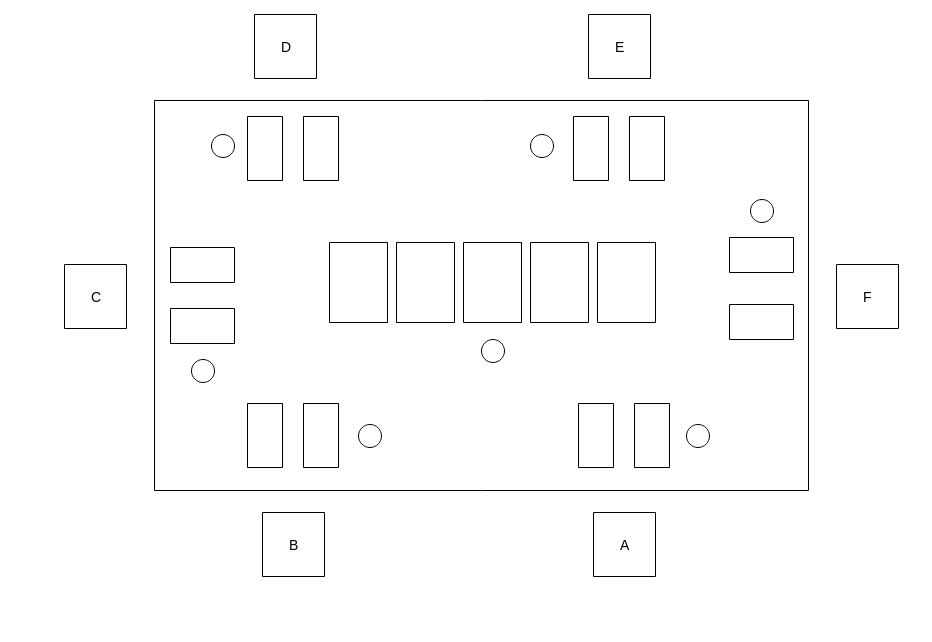
\includegraphics[width=\linewidth]{../images/initialgui.png}}
    \caption{Initial GUI mockup}%
    \label{fig:initialgui}
\end{figure}

This is a very standard design which cannot be varied much. All players have
two cards, a current bet, and a total amount of chips. As you may notice
in Figure~\ref{fig:initialgui} there is no label for the players total amount
of chips. This was instead decided to be stored as part of the name component,
as it makes for much less visual noise. The player labelled `A', is the
users player. He/she will always be seated here, and the other players will
be rotated around the board from their perspective. That is, every single
player A through F will appear to be in seat A from their own point of view.
The GUI is player centric. The relative positions, however will not be 
modified. Player A will always have player B to their left and Player F to 
their right, no matter where they visually appear to be. Of course, this has 
been implemented to not affect how the gameplay works, as the ordering of 
players is maintained, it is simply the visual representation of the players 
which is being manipulated.

The players need some way to interact with the game, and simple buttons which 
lie under the poker table were used for this. The raise button brought some 
complications, as the user has to enter a valid integer to increase the current
bet to. Some constraints are placed on this parameter.

\newpage

\begin{itemize}
\item The user must have enough chips to make the raise
\item The user must raise by at least the minimum raise
\item The raise must be an integer, not fractional
\end{itemize}

It was decided to use a separate window with a slider to handle the above
reasons. A slider has a minimum, and a maximum. This prevents the user from
both raising too little, and too much. And, by setting a slide interval, it
prevents the user selecting a non integer.

\begin{figure}[h]
    \centering
    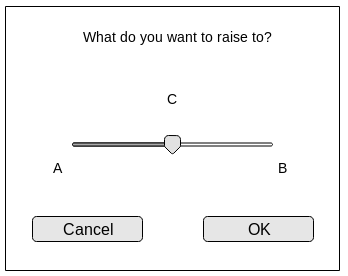
\includegraphics[width=0.5\linewidth]{../images/raisewindow.png}
    \caption{The Raise Window, where A is the minimum raise, B is the maximum
             raise, and C is the currently selected raise value}%
    \label{fig:raisewindow}
\end{figure}

However, in the implementation of this, it was found that when displaying
the selected value, despite the steps being integer steps of one, 
fractional values could arise due to inherent errors in floating point 
mathematics. This was solved by simply taking the raw slider value, and 
casting it to an integer variable. This variable was then used for displaying 
the current users selection, and for the program to take as the chosen value 
once the `OK' button had been selected. Figure~\ref{fig:raisewindow} shows the 
raise window, where A is the minimum value, B is the maximum value, and C is 
the current value. It should be noted that these values are denoted in chips,
and no particular currency is implied, though most casinos usually peg a
fiat value to a chip.

\begin{figure}
    \centering
    \begin{subfigure}[h]{0.4\textwidth}
        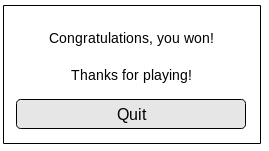
\includegraphics[width=\textwidth]{../images/winscreen.png}
        \caption{The Win Window}%
        \label{fig:winwindow}
    \end{subfigure}
    \begin{subfigure}[h]{0.4\textwidth}
        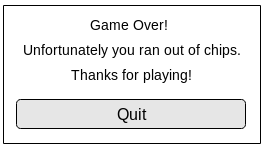
\includegraphics[width=\textwidth]{../images/lossscreen.png}
        \caption{The Loss Window}%
        \label{fig:losswindow}
    \end{subfigure}
    \caption{The Game Over Windows}\label{fig:gameoverwindows}
\end{figure}

Finally, there were elements needed for when a player either wins the game,
by the other players being eliminated for running out of chips, or when a
player loses, by being eliminated themselves. These took the form of simple
windows with configurable text, and a quit button. Both the win window
and the loss window use the same component, with only differing text. This
keeps the GUI consistent, and thus increases user acceptance.

Once the mockups had been completed the GUI was implemented in QtQML,
and hooked up to the Haskell code so it was fully usable and could be used
to test the poker game. Figure~\ref{fig:actualgui} shows the GUI in use,
with 6 players participating in a game. 

\begin{figure}[h]
    \centering
    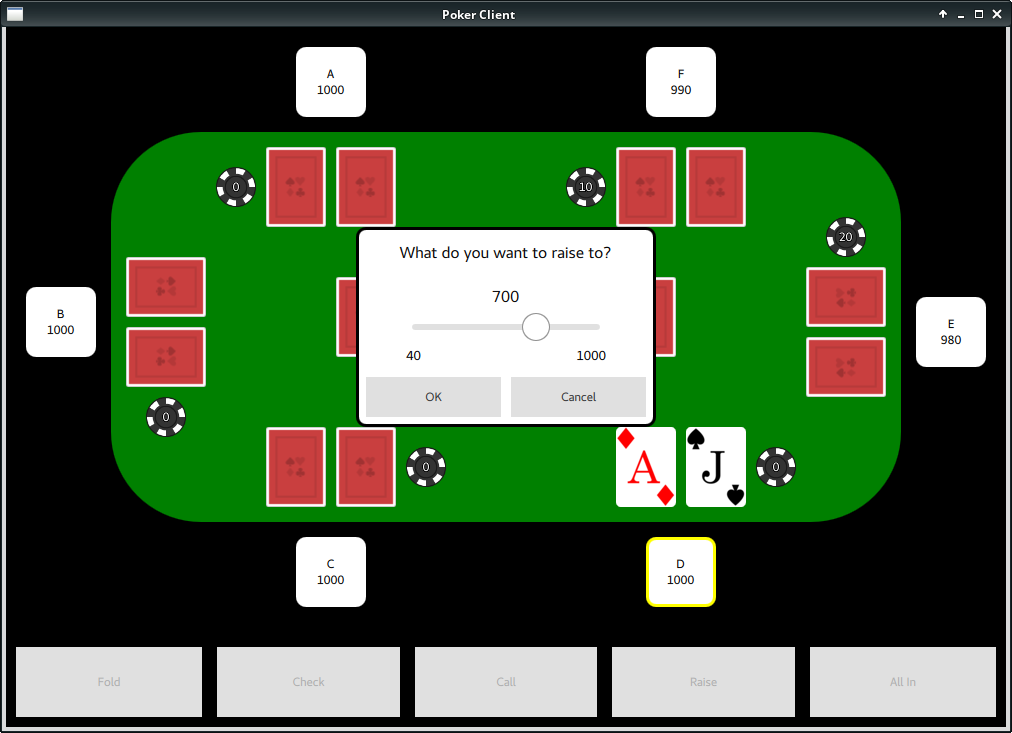
\includegraphics[width=\textwidth]{../images/actualgui.png}
    \caption{The initial implemented GUI}%
    \label{fig:actualgui}
\end{figure}

You can also see the implemented raise window in this image. Aside from the 
obvious card and poker chip assets, and colours, the implemented GUI is 
essentially the same as the mockup. One difference that was decided upon 
adding whilst testing, was a yellow border around the current player, so users 
would know how long it was until it was their turn. 

One feature of note is button fading. When buttons are unavailable, for
example if it's not the players turn, or a certain action would be invalid,
the buttons are greyed out, and unclickable. When actions become available,
they are clickable and fully coloured. This is an easy way to let players
know the valid actions whilst keeping the GUI consistent. Faded and non faded
buttons can be seen in figure~\ref{fig:guiwithconsole}.

Another modification considered making was adding a dealer chip. Whilst
online poker does not have an actual player who deals the cards, and indeed
in real life poker the dealer is often not an actual player, the concept of
a dealer is still used.

Each round, the dealer progresses, and the player to
the left of the dealer is the player who bets first. In the preflop, this
player has to play a forced blind, but once in the flop and beyond, this player
gets to bet first, which is of some strategic importance. 

For these reasons, a dealer chip would seem obvious, however it was decided
against, because it both clutters the GUI, and the dealer can still be
recognised by simply observing who plays the small blind, and retaining this
information, knowing the dealer progresses once to the left each full round.
In the above screenshot for example, the dealer can be identified to be A,
as the player to his left has played a small blind of 10 chips.

One modification that was added after the initial implementation was a text
console. This was used because some important information was difficult to 
display graphically, had to be interpreted very quickly, or was useful to be 
consulted at a later point in the game. The text console allowed messages such 
as bet history and hand values to be constantly visible to allow players to 
digest at their own pace.

\begin{figure}[h]
    \centering
    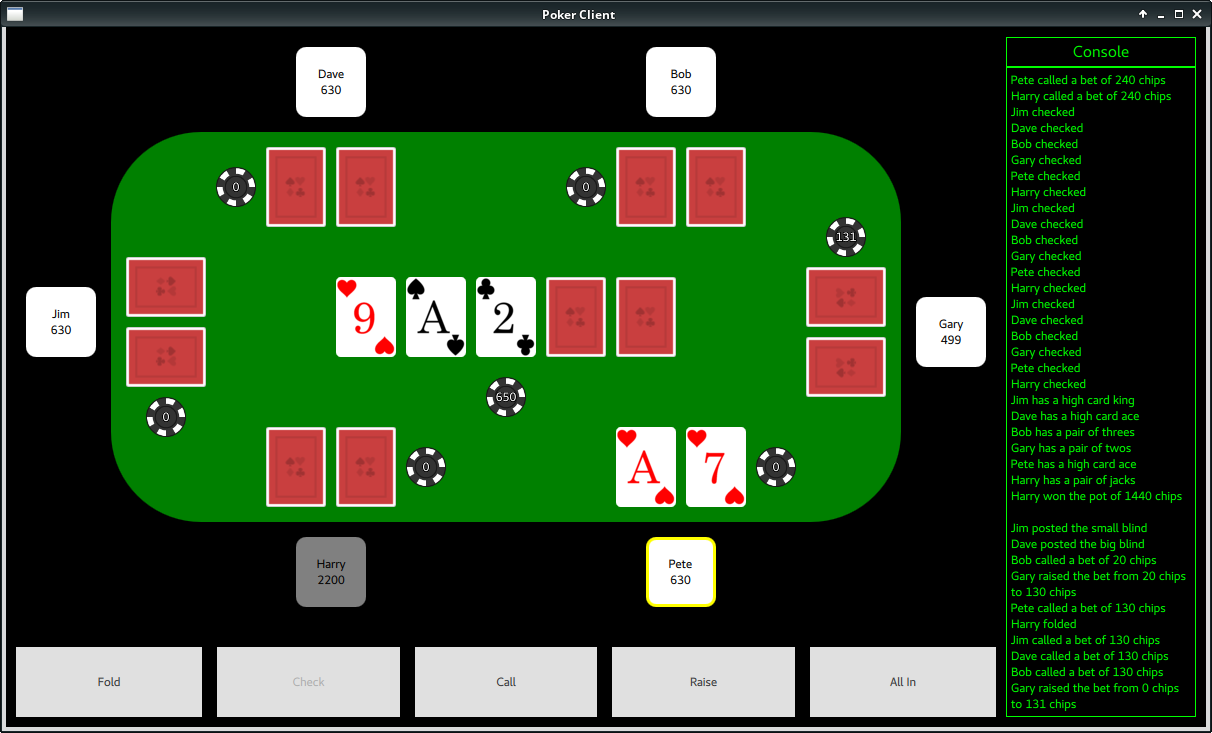
\includegraphics[width=\textwidth]{../images/guiwithconsole.png}
    \caption{The GUI with text console}%
    \label{fig:guiwithconsole}
\end{figure}
